\section{Citation Fidelity}
\label{sec:citations}

The rubric in \Cref{sec:experiments} counted a claim as supported when it carried a citation. It did not check whether the cited source says what the claim says. Attribution studies of generative search engines find that this check matters: in \citet{liu2023verifiability}, a quarter of citations did not support their sentence. This section measures it for \sys{}, finds that the evaluated reports fail it, traces the failure to two specific steps in the pipeline, and fixes them.

\subsection{A lexical attribution test}
For every sentence with bracketed citations, the test ranks all sources available to the document by TF-IDF cosine similarity \citep{salton1988termweighting} between the sentence and the source text, and records the rank of each cited source as a percentile (0 for the best match, 1 for the worst). If citations point to the sources a claim was written from, cited sources rank near the top. If citation numbers are scrambled, their percentile is uniform on $[0, 1]$, with median 0.5. Two summary statistics are reported: the median percentile of cited sources, and the share of claims whose single best-matching source is among those cited, against the share expected by chance. The test needs no model calls and runs on every report. It is lexical, so a source that paraphrases a claim in different words can rank low; the validation below measures how much this matters.

\paragraph{Validation.}
The leaf answers of the logged run (\Cref{app:dag}) are written by one model call directly from the retrieved excerpts they cite, so their citations are correct by construction. Against all \atValMeanCandidates{} sources of the run, the cited source is the best match for \atValBestCited{} of leaf claims, against \atValBestChance{} by chance, and the median percentile of cited sources is \atValMedianPct{} (95\% interval \atValPctLo--\atValPctHi). The evaluated reports cite full web pages rather than excerpts, so the test was repeated with the full text of the logged run's pages, fetched for this analysis: on the \atValPagesMeanCandidates{} pages that returned usable text, the cited page is the best match for \atValPagesBestCited{} of claims (chance \atValPagesBestChance). The test separates correct from scrambled citations clearly on both kinds of text.

\begin{table}[t]
\centering
\small
\resizebox{\linewidth}{!}{\begin{tabular}{lrrrrr}
\toprule
Setting & Claim--source pairs & Median rank percentile & Top-3 hit rate & Chance & Best match cited \\
\midrule
Leaf answers, own numbering & 63 & 0.04 [0.00, 0.08] & 0.83 & 0.12 & 0.96 (chance 0.10) \\
Leaf answers, own numbering, full pages & 24 & 0.00 [0.00, 0.11] & 0.88 & 0.30 & 0.84 (chance 0.13) \\
Leaf answers as a parent reads them, global numbering & 63 & 0.04 [0.00, 0.08] & 0.83 & 0.12 & 0.96 (chance 0.10) \\
Leaf answers as a parent read them, original pipeline & 63 & 0.12 [0.08, 0.16] & 0.49 & 0.12 & 0.52 (chance 0.10) \\
Final report, logged run & 173 & 0.48 [0.44, 0.52] & 0.06 & 0.12 & 0.04 (chance 0.10) \\
Evaluated reports, all listed sources & 491 & 0.47 [0.40, 0.53] & 0.18 & 0.14 & 0.14 (chance 0.10) \\
Evaluated reports, cited sources only & 491 & 0.43 [0.40, 0.50] & 0.56 & 0.51 & 0.41 (chance 0.36) \\
\bottomrule
\end{tabular}
}
\caption{Attribution of cited claims. Each row ranks every available source by lexical similarity to each cited claim. The median rank percentile of the cited sources is 0 if they are always the best match and 0.5 if citations are random (95\% bootstrap interval in brackets). The top-3 hit rate is the share of cited sources ranked in the top three; chance is its expected value under random citation. The last column is the share of claims whose best match is cited.}
\label{tab:attribution}
\end{table}

\begin{figure}[t]
\centering
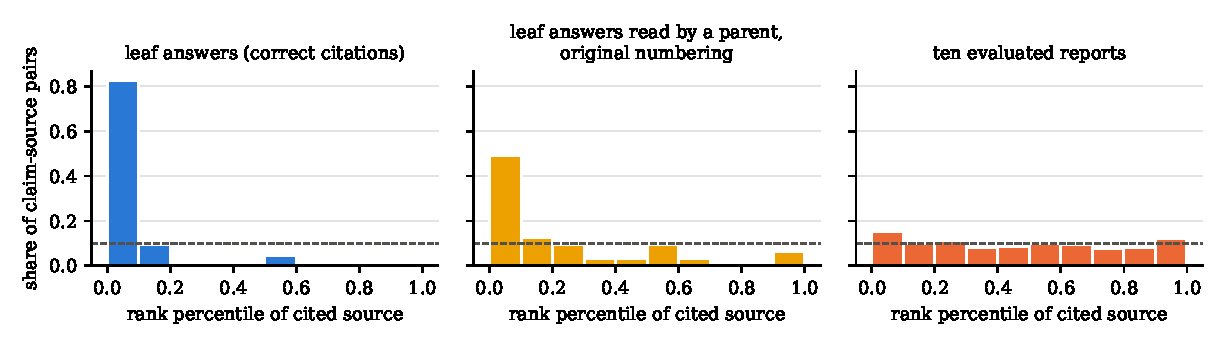
\includegraphics[width=\linewidth]{figs/attribution.pdf}
\caption{Rank percentile of each cited source among all available sources. Correct citations pile up at 0 (left). The evaluated reports are flat, as random citations would be (right). The middle panel shows the leaf answers as a parent node in the repository version read them (\Cref{sec:mechanism}). The dashed line marks the uniform distribution.}
\label{fig:attribution}
\end{figure}

\subsection{Results}
\Cref{tab:attribution} and \Cref{fig:attribution} give the results. In the ten evaluated reports, the \atEvalClaims{} cited claims carry \atEvalPairs{} claim--source pairs. The median percentile of the cited sources among all listed sources is \atEvalMedianPct{} (\atEvalPctLo--\atEvalPctHi), indistinguishable from 0.5, and the claim's best match is cited for \atEvalBestCited{} of claims against \atEvalBestChance{} by chance. Restricting the candidates to the sources the report actually cites, a median of \atEvalCitedMeanCandidates{} per report, the best match is cited for \atEvalCitedBestCited{} of claims against \atEvalCitedBestChance{} by chance. The final report of the logged run, produced with the same report-writing step, is also at chance (median percentile \atLogMedianPct). By this test, the citations in the evaluated reports carry almost no information about which source supports which claim.

Two cases from the theism report show what this looks like. A bullet stating that ``non-theistic systems such as Confucianism, Buddhism, and Stoicism achieved moral stability'' without divine law cites five sources, all of them arguments for the existence of God from the moral law. A bullet on ancient Egyptian, Israelite, and Vedic societies cites ``A Beginner's Guide to the Moral Argument.'' The claims may well be true; the cited sources are not where they came from.

\subsection{Mechanism}
\label{sec:mechanism}
The code that produced the evaluated reports is not public (\Cref{app:changes}), but the repository version from a week earlier is, together with a run it produced, and it loses provenance at two steps. Both are consistent with the symptoms of the evaluated reports, though they cannot be confirmed in that version's code.

\paragraph{Local numbers read in a merged list.}
A leaf answer cites its own sources as [1] to [$k$]. When a parent is composed, the repository version merges its children's sources into one deduplicated list numbered [1] to [$m$] and gives the synthesis model this list with the instruction to cite by its numbers, but it passes the children's answers with their original leaf-local numbers. A ``[1]'' copied from the second child therefore points to the first child's first source. The middle rows of \Cref{tab:attribution} replay this on the logged run. Read in the parent's merged list, the leaf claims' citations still hit the best match for \atOldBestCited{} of claims, the correct ones from each parent's first child, but no longer the \atValBestCited{} they had in their own numbering. Every level of the DAG applies this scrambling again.

\paragraph{Node identifiers instead of sources.}
The composition instructions generated in Phase 1 tell the synthesis model to credit children by node identifier so that dependencies can be traced, while the synthesis prompt tells it to cite sources by number. In the logged run, \dagParents{} nodes were composed, counting the root. Three of them, the root among them, followed the composition instructions and wrote references such as ``(node\_3)'' after their claims, with no source numbers at all; one cited by number. The report writer then receives a root answer without source citations and an instruction to cite by number, and assigns numbers it has no basis for, which is why the logged report is at chance.

\subsection{Fix}
The released code makes provenance explicit. Every source receives one global number when any node first retrieves it, and leaf answers are rewritten from local to global numbers before they are stored, so children and parent share one numbering and the report's bibliography uses it too. After composition, node identifiers in the parent's answer are replaced by the global citations of those children, and numbers outside the parent's sources are removed. The synthesis prompt and the composition-instruction prompt both now say to cite sources by number and never by node. The lexical test above is included as an audit that can flag claims whose cited sources rank in the bottom half. Replayed on the logged run, the leaf claims keep their attribution under the new numbering (\atFixBestCited{} best-match rate, the same as the leaves themselves). Whether the report writer then preserves it end to end requires new runs, which are not part of this study; the test makes that check cheap.

\subsection{Implications}
The supported-claims rate in \Cref{tab:human} counted citation markers, so it measures how consistently \sys{} attaches citations, which it does more densely than STORM (\Cref{sec:analysis}), not whether its claims are supported by what they cite. The evaluated reports should not be read as better grounded than the baselines; the evaluation does not show that. The same test applies to any system with inline citations; STORM's exports lacked URLs and Deep Research's reports were not retained, so neither baseline could be checked here.
